\documentclass[a4paper]{article}

\usepackage[T1]{fontenc}
\usepackage[english]{babel}
\usepackage[utf8]{inputenc}
\usepackage [autostyle, english=american]{csquotes}
\MakeOuterQuote{"}
\usepackage[maxbibnames=99,style=numeric,sorting=none]{biblatex}
\addbibresource{bib.bib}
\usepackage[
    pdfusetitle,
    pdfkeywords={Line Generalization,Cartographic Line Generalization,Wang--M{\"u}ller},
    pdfborderstyle={/S/U/W 0} % /S/U/W 1 to enable reasonable decorations
]{hyperref}
\usepackage{enumitem}
\usepackage[toc,page,title]{appendix}
\usepackage{caption}
\usepackage{subcaption}
\usepackage{gensymb}
\usepackage{units}
\usepackage{varwidth}
\usepackage{tabularx}
\usepackage{float}
\usepackage{tikz}
\usepackage{fancyvrb}
%\usepackage{charter}

\iftrue
% requires minted
\usepackage{minted}
\newcommand{\inputcode}[2]{\inputminted[fontsize=\small]{#1}{#2}}
\else
% does not require minted
\usepackage{verbatim}
\newcommand{\inputcode}[2]{\verbatiminput{#2}}
\usepackage{setspace}
\doublespacing
\fi

\gdef\VCDescribe{2021-05-08 (revision a627e2097554)}%

\newcommand{\smallAngle}{\frac{\pi}{4}}
\newcommand{\isolationThreshold}{0.50}


% for layout debugging
\usepackage{layouts}

\newcommand{\onpage}[1]{\ref{#1} on page~\pageref{#1}}
\newcommand{\titlecite}[1]{\citetitle{#1}\cite{#1}}
\newcommand{\DP}{Douglas \& Peucker}
\newcommand{\VW}{Visvalingam--Whyatt}
\newcommand{\WM}{Wang--M{\"u}ller}
\newcommand{\MYTITLE}{Cartographic Line Generalization (example of rivers)}
\newcommand{\MYAUTHOR}{Motiejus Jakštys}

\title{\MYTITLE}
\author{\MYAUTHOR}
\date{\VCDescribe}

\begin{document}

\begin{titlepage}
    \begin{center}
        
\includegraphics[width=0.4\textwidth]{vu}

        \huge
        \textbf{\MYTITLE} \\[4ex]

        \LARGE
        \textbf{\MYAUTHOR} \\[8ex]

        \vfill

        A thesis presented for the degree of\\
        Master in Cartography \\[3ex]

        \large
        \VCDescribe
    \end{center}
\end{titlepage}

\begin{abstract}
\label{sec:abstract}
Current open-source line generalization solutions have their roots in
    mathematics and geometry, and are not fit for natural objects like rivers
    and coastlines. This paper discusses our implementation of {\WM}'s algorithm
    under and open-source license, explains things that we would had
    appreciated in the original paper and compares our results to different
    generalization algorithms.
\end{abstract}

\newpage

\tableofcontents
\listoffigures

\newpage

\section{Introduction}
\label{sec:introduction}

\iffalse
NOTICE: this value should be copied to layer2img.py:TEXTWIDTH, so dimensions
of inline images are reasonable.

Textwidth in cm: {\printinunitsof{cm}\prntlen{\textwidth}}
\fi

When creating small-scale maps, often the detail of the data source is greater
than desired for the map. While many features can be removed or simplified, it
is more tricky with natural features that have many bends, like coastlines,
rivers and forest boundaries.

To create a small-scale map from a large-scale data source, features need to be
generalized: detail should be reduced. While performing the generalization, it
is important to retain the "defining" shape of the original feature. Otherwise,
if the generalized feature looks too different than the original, the result
will look unrealistic.

For example, if a river is nearly straight, it should be nearly straight after
generalization, otherwise a too straightened river will look like a canal.
Conversely, if the river is highly wiggly, the number of bends should be
reduced, but not removed altogether.

Generalization problem for other objects can often be solved by other
non-geometric means:

\begin{itemize}
    \item Towns and cities can be filtered and generalized by number of
        inhabitants.
    \item Roads can be eliminated by the road length, number of lanes, or
        classification of the road (local, regional, international).
\end{itemize}

To sum up, natural line generalization problem can be viewed as a task of
finding a delicate balance between two competing goals:

\begin{itemize}
    \item Reduce detail by removing or simplifying "less important" features.
    \item Retain enough detail, so the original is still recognize-able.
\end{itemize}

Given the discussed complexities, a fine line between under-generalization
(leaving object as-is) and over-generalization (making a straight line) needs
to be found. Therein lies the complexity of generalization algorithms: all have
different trade-offs.

\section{Literature review and problematic}
\label{sec:literature-review}

A number of cartographic line generalization algorithms have been researched.
The "classical" ones are {\DP}\cite{douglas1973algorithms} and
{\VW}\cite{visvalingam1993line} in combination with
Chaikin's\cite{chaikin1974algorithm}.

This section reviews the classical ones, which, besides being around for a long
time, offer easily accessible implementations, as well as more modern ones,
which only theorize, but do not provide an implementation.

\subsection{Available algorithms}

\subsubsection{{\DP}, {\VW} and Chaikin's}

{\DP}\cite{douglas1973algorithms} and {\VW}\cite{visvalingam1993line} are
"classical" line generalization computer graphics algorithms. They are
relatively simple to implement, require few runtime resources. Both of them
accept only a single parameter, based on desired scale of the map, which makes
them straightforward to adjust for different scales.

Both algorithms are part of PostGIS, a free-software GIS suite:
\begin{itemize}
    \item {\DP} via
        \href{https://postgis.net/docs/ST_Simplify.html}{PostGIS \texttt{ST\_Simplify}}.

    \item {\VW} via
        \href{https://postgis.net/docs/ST_SimplifyVW.html}{PostGIS \texttt{SimplifyVW}}.
\end{itemize}

It may be worthwhile to post-process those through a widely available Chaikin's
line smoothing algorithm\cite{chaikin1974algorithm} via
\href{https://postgis.net/docs/ST_ChaikinSmoothing.html}{PostGIS
\texttt{ST\_ChaikinSmoothing}}.

To use in generalization examples, we will use two rivers: Šalčia and Visinčia.
Figure~\ref{fig:salvis-25} illustrates the original two rivers without any
processing.

These rivers were chosen, because they have both large and small bends, and
thus convenient to analyze for both small and large scale generalization.

\begin{figure}[h]
    \centering
    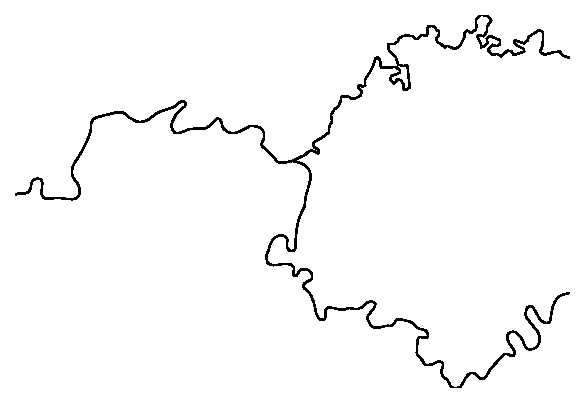
\includegraphics[width=\textwidth]{salvis-25k}
    \caption{Example rivers for visual tests (1:25000).}
    \label{fig:salvis-25}
\end{figure}

\begin{figure}[h]
    \centering
    \begin{subfigure}[b]{.49\textwidth}
        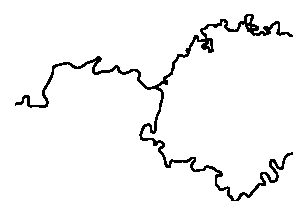
\includegraphics[width=\textwidth]{salvis-50k}
        \caption{Example scaled 1:50000.}
    \end{subfigure}
    \hfill
    \begin{subfigure}[b]{.49\textwidth}
        \centering
        
\includegraphics[width=.2\textwidth]{salvis-250k}
        \caption{Example scaled 1:250000.}
    \end{subfigure}
    \caption{Down-scaled original river (1:50000 and 1:250000).}
    \label{fig:salvis-50-250}
\end{figure}

Same rivers, unprocessed, but with higher density (scales 1:50000 and 1:250000)
are depicted in figure~\onpage{fig:salvis-50-250}. Some river features are so
compact that a reasonably thin line depicting the river is touching itself,
creating a thicker line. As a result, generalization for this river for a
smaller scale is worthy.

\begin{figure}[h]
    \centering
    \begin{subfigure}[b]{.49\textwidth}
        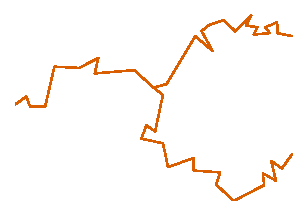
\includegraphics[width=\textwidth]{salvis-douglas-64-50k}
        \caption{Using {\DP}}
    \end{subfigure}
    \hfill
    \begin{subfigure}[b]{.49\textwidth}
        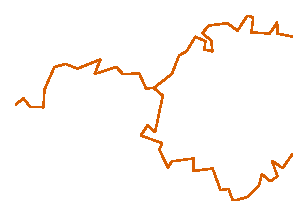
\includegraphics[width=\textwidth]{salvis-visvalingam-64-50k}
        \caption{Using {\VW}}
    \end{subfigure}
    \caption{Generalized using classical algorithms (1:50000).}
    \label{fig:salvis-generalized-50k}
\end{figure}


Figure~\onpage{fig:salvis-generalized-50k} illustrates the same river bend, but
generalized using {\DP} and {\VW} algorithms. The resulting lines are jagged,
thus the resulting line looks unlike a real river. To smoothen the jaggedness,
traditionally, Chaikin's\cite{chaikin1974algorithm} is applied after
generalization, illustrated in
figure~\onpage{fig:salvis-generalized-chaikin-50k}.

\begin{figure}[h]
    \centering
    \begin{subfigure}[b]{.49\textwidth}
        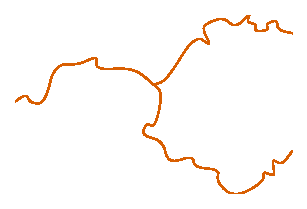
\includegraphics[width=\textwidth]{salvis-douglas-64-chaikin-50k}
        \caption{Using {\DP} and Chaikin's}
    \end{subfigure}
    \hfill
    \begin{subfigure}[b]{.49\textwidth}
        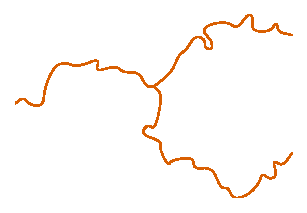
\includegraphics[width=\textwidth]{salvis-visvalingam-64-chaikin-50k}
        \caption{Using {\VW} and Chaikin's}
    \end{subfigure}
    \caption{Generalized and smoothened river (1:50000).}
    \label{fig:salvis-generalized-chaikin-50k}
\end{figure}

There are a few problems with {\VW} and {\DP} immediately visible in
figure~\onpage{fig:salvis-generalized-chaikin-50k}:

\begin{itemize}
    \item problem 1
    \item problem 2
\end{itemize}

Therefore, a more robust generalization algorithm is worthwhile for lookout.

\subsubsection{Modern approaches}

Due to their simplicity and ubiquity, {\DP} and {\VW} have been established as
go-to algorithms for line generalization. During recent years, alternatives
have emerged. These modern replacements fall into roughly two categories:

\begin{itemize}

    \item Cartographic knowledge was encoded to an algorithm (bottom-up
        approach). One among these are \titlecite{wang1998line}, also known
        as {\WM}'s algorithm.

    \item Mathematical shape transformation which yields a more cartographic
        result. E.g. \titlecite{jiang2003line},
        \titlecite{dyken2009simultaneous}, \titlecite{mustafa2006dynamic},
        \titlecite{nollenburg2008morphing}.

\end{itemize}

Authors of most of the aforementioned articles have implemented the
generalization algorithm, at least to generate the illustrations in the
articles. However, code is not available for evaluation with a desired data
set, much less for use as a basis for creating new maps. To author's knowledge,
{\WM}\cite{wang1998line} is available in a commercial product, but requires a
purchase of the commercial product suite, without a way to license the
standalone algorithm.

Lack of robust openly available generalization algorithm implementations poses
a problem for map creation with free software: there is not a similar
high-quality simplification algorithm to create down-scaled maps, so any
cartographic work, which uses line generalization as part of its processing,
will be of sub-par quality. We believe that availability of high-quality
open-source tools is an important foundation for future cartographic
experimentation and development, thus it it benefits the cartographic society
as a whole.

{\WM}'s commercial availability signals something about the value of the
algorithm: at least the authors of the commercial software suite deemed it
worthwhile to include it. However, not everyone has access to the commercial
software suite, access to funds to buy the commercial suite, or access to the
operating system required to run the commercial suite. PostGIS, in contrast, is
free on itself, and runs on free platforms. Therefore, algorithm
implementations that run on PostGIS or other free platforms are useful to a
wider cartographic society than proprietary ones.

\subsection{Problematic with generalization of rivers}

\section{Methodology}
\label{sec:methodology}

The original {\WM}'s algorithm \cite{wang1998line} leaves something to be
desired for a practical implementation: it is not straightforward to implement
the algorithm from the paper alone.

Explanations in this document are meant to expand, rather than substitute, the
original description in {\WM}. Therefore familiarity with the original paper is
assumed, and, for some sections, having the original close-by is necessary to
meaningfully follow this document.

This paper describes {\WM} in detail that is more useful for anyone who wishes
to follow the algorithm implementation more closely: each section is expanded
with additional commentary, and richer illustrations for non-obvious steps. In
many cases, corner cases are discussed and clarified.

Assume Euclidean geometry throughout this document, unless noted otherwise.

\subsection{Vocabulary and terminology}
\label{sec:vocab}

This section defines vocabulary and terms as defined in the rest of the paper.

\begin{description}

    \item[Vertex] is a point on a plane, can be expressed by a pair of $(x,y)$
        coordinates.

    \item[Line Segment (or Segment)] joins two vertices by a straight line. A
        segment can be expressed by two coordinate pairs: $(x_1, y_1)$ and
        $(x_2, y_2)$. Line Segment and Segment are used interchangeably
        throughout the paper.

    \item[Line], or \textsc{linestring}, represents a single linear feature in
        the real world. For example, a river or a coastline.

        Geometrically, A line is a series of connected line segments, or,
        equivalently, a series of connected vertices. Each vertex connects to
        two other vertices, except those vertices at either ends of the line:
        these two connect to a single other vertex.

    \item[Bend] is a subset of a line that humans perceive as a curve. The
        geometric definition is complex and is discussed in
        section~\onpage{sec:definition-of-a-bend}.

    \item[Baseline] is a line between bend's first and last vertex.

    \item[Sum of inner angles] TBD.

    \item[Algorithmic Complexity] also called \textsc{big o notation}, is a
        relative measure to explain how long will the algorithm run depending
        on it's input. For example, given $n$ objects and time complexity of
        $O(n)$, the time it takes to execute the algorithm is proportional to
        $n$. Conversely, if complexity is $O(n^2)$, then the time it takes to
        execute the algorithm is quadratic. $O$ notation was first suggested by
        Bachmann\cite{bachmann1894analytische} and
        Laundau\cite{landau2000handbuch} in late XIX'th century, and adopted
        for computer science by Donald Knuth\cite{knuth1976big} in 1970s.

\end{description}

\subsection{Radians and Degrees}

This document contains a few constant angles expressed in radians.
Table~\ref{table:radians} summarizes some of the values used in this document
and the implementation.

\begin{table}[h]
    \centering
    \begin{tabular}{|c|c|c|c|c|c|c|}
        \hline
        Degrees & $30^\circ$          & $45^\circ$          & $90^\circ$          & $180^\circ$ & $360^\circ$ \\
        \hline
        Radians & $\nicefrac{\pi}{6}$ & $\nicefrac{\pi}{4}$ & $\nicefrac{\pi}{2}$ & $\pi$       & $2\pi$ \\
        \hline
    \end{tabular}
    \caption{Some angular degree and radian values mentioned in this article.}
    \label{table:radians}
\end{table}

\subsection{Automated tests}
\label{sec:automated-tests}

As part of the algorithm realization, an automated test suite has been
developed. Shapes to test each function have been hand-crafted and expected
results have been manually calculated. The test suite executes parts of the
algorithm against a predefined set of geometries, and asserts that the output
matches the resulting hand-calculated geometry.

The full set of test geometries is visualized in
figure~\ref{fig:test-figures}.

\begin{figure}[h]
    \centering
    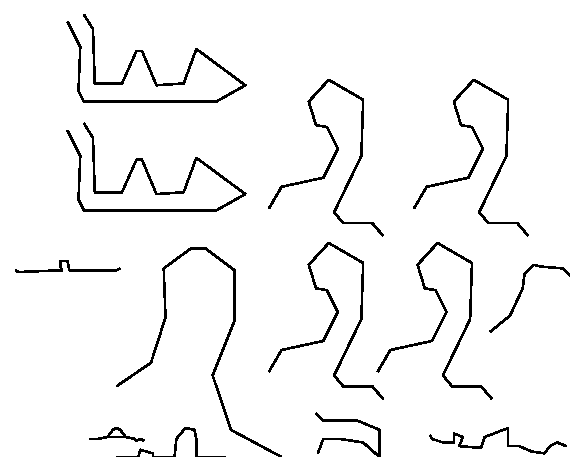
\includegraphics[width=\textwidth]{test-figures}
    \caption{Line geometries for automated test cases.}
    \label{fig:test-figures}
\end{figure}

The full test suite can be executed with a single command, and completes in a
few seconds. Having an easily accessible test suite boosts confidence that no
unexpected bugs have snug in while modifying the algorithm.

\subsection{Reproducing generalizations in this paper}
\label{sec:reproducing-the-paper}

It is widely believed that the ability to reproduce the results of a published
study is important to the scientific community. In practice, however, it is
often hard to impossible: research methodologies, as well as algorithms
themselves, are explained in prose, which, due to the nature of the non-machine
language, lends itself to inexact interpretations.

This article, besides explaining the algorithm in prose, \emph{includes} the
program of the algorithm in a way that can be executed on reader's workstation.
On top of it, all the illustrations in this paper are generated using that
algorithm, from a predefined list of test geometries (test geometries were
explained in section~\ref{sec:automated-tests}).

Instructions how to re-generate all the visualizations are found in
appendix~\ref{sec:code-regenerate}. The visualization code serves as a good
example reference for anyone willing to start using the algorithm.

\section{Description of the implementation}

Like alluded in section~\ref{sec:introduction}, {\WM} paper skims over
certain details, which are important to implement the algorithm. This section
goes through each algorithm stage, illustrating the intermediate steps and
explaining the author's desiderata for a more detailed description.

Illustrations of the following sections are extracted from the automated test
cases, which were written during the algorithm implementation (as discussed in
section~\onpage{sec:automated-tests}).

Illustrated lines are black. Bends themselves are linear features.
Discriminating between bends in illustrations might be tricky, because
sometimes a single \textsc{line segment} can belong to two bends.

Given that, there is another way to highlight bends in a schematic drawing: by
converting them to polygons and by altering their background colors. It works
as follows:

\begin{itemize}
    \item Join the first and last vertices of the bend, creating a polygon.
    \item Color the polygons using distinct colors.
\end{itemize}

This type of illustration works quite well, since polygons created from bends
are almost never overlapping, and discriminating different backgrounds is
easier than discriminating different line shapes or colors.

\subsection{Definition of a Bend}
\label{sec:definition-of-a-bend}

The original article describes a bend as:

\begin{displaycquote}{wang1998line}
    A bend can be defined as that part of a line which contains a number of
    subsequent vertices, with the inflection angles on all vertices included in
    the bend being either positive or negative and the inflection of the bend's
    two end vertices being in opposite signs.
\end{displaycquote}

While it gives a good intuitive understanding of what the bend is, this section
provides more technical details. Here are some non-obvious characteristics that
are necessary when writing code to detect the bends:

\begin{itemize}
    \item End segments of each line should also belong to bends. That way, all
        segments belong to 1 or 2 bends.

    \item First and last segments of each bend (except for the two end-line
        segments) are also the first vertex of the next bend.
\end{itemize}

Properties above may be apparent when looking at illustrations at this article
or reading here, but they are nowhere as such when looking at the original
article.

Figure~\ref{fig:fig8-definition-of-a-bend} illustrates article's figure 8,
but with bends colored as polygons: each color is a distinctive bend.

\begin{figure}[h]
    \centering
    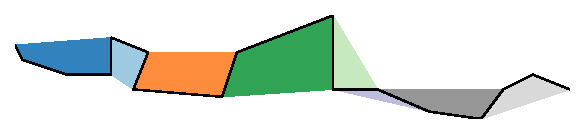
\includegraphics[width=\textwidth]{fig8-definition-of-a-bend}
    \caption{Originally figure 8: detected bends are highlighted.}
    \label{fig:fig8-definition-of-a-bend}
\end{figure}

\subsection{Gentle Inflection at End of a Bend}

The gist of the section is in the original article:

\begin{displaycquote}{wang1998line}
    But if the inflection that marks the end of a bend is quite small, people
    would not recognize this as the bend point of a bend
\end{displaycquote}

Figure~\ref{fig:fig5-gentle-inflection} visualizes original paper's figure 5,
when a single vertex is moved outwards the end of the bend.

\begin{figure}[h]
    \centering
    \begin{subfigure}[b]{.49\textwidth}
        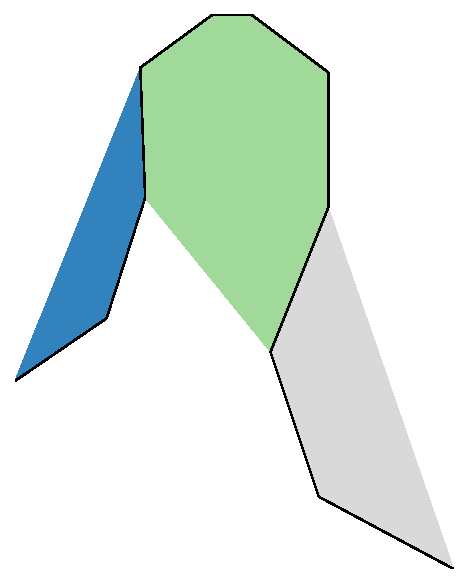
\includegraphics[width=\textwidth]{fig5-gentle-inflection-before}
        \caption{Before applying the inflection rule.}
    \end{subfigure}
    \hfill
    \begin{subfigure}[b]{.49\textwidth}
        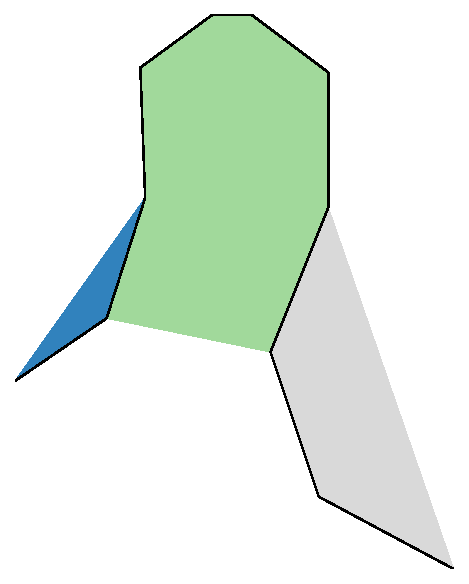
\includegraphics[width=\textwidth]{fig5-gentle-inflection-after}
        \caption{After applying the inflection rule.}
    \end{subfigure}
    \caption{Originally figure 5: gentle inflections at the ends of the bend.}
    \label{fig:fig5-gentle-inflection}
\end{figure}

The illustration for this section was clear, but insufficient: it does not
specify how many vertices should be included when calculating the end-of-bend
inflection. The iterative approach was chosen --- as long as the angle is "right"
and the distance is decreasing, the algorithm should keep re-assigning vertices
to different bends; practically not having an upper bound on the number of
iterations.

To prove that the algorithm implementation is correct for multiple vertices,
additional example was created, and illustrated in
figure~\ref{fig:inflection-1-gentle-inflection}: the rule re-assigns two
vertices to the next bend.

\begin{figure}[h]
    \centering
    \begin{subfigure}[b]{.49\textwidth}
        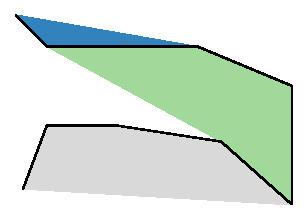
\includegraphics[width=\textwidth]{inflection-1-gentle-inflection-before}
        \caption{Before applying the inflection rule.}
    \end{subfigure}
    \hfill
    \begin{subfigure}[b]{.49\textwidth}
        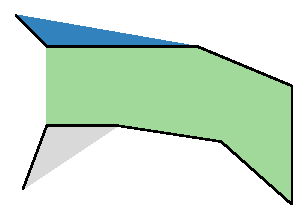
\includegraphics[width=\textwidth]{inflection-1-gentle-inflection-after}
        \caption{After applying the inflection rule.}
    \end{subfigure}
    \caption{Gentle inflection at the end of the bend when multiple vertices
    are moved.}
    \label{fig:inflection-1-gentle-inflection}
\end{figure}

Note that to find and fix the gentle bends' inflections, the algorithm should
run twice, both ways. Otherwise, if it is executed only one way, the steps will
fail to match some bends that should be adjusted. Current implementation works
as follows:

\begin{enumerate}
    \item Run the algorithm from beginning to the end.
    \item \label{rev1} Reverse the line and each bend.
    \item Run the algorithm again.
    \item \label{rev2} Reverse the line and each bend.
    \item Return result.
\end{enumerate}

Reversing the line and its bends is straightforward to implement, but costly:
the two reversal steps cost additional time and memory. The algorithm could be
made more optimal with a similar version of the algorithm, but the one which
goes backwards. In this case, steps \ref{rev1} and \ref{rev2} could be spared,
that way saving memory and computation time.

The "quite small angle" was arbitrarily chosen to $\smallAngle$.

\subsection{Self-line Crossing When Cutting a Bend}

When bend's baseline crosses another bend, it is called self-crossing.
Self-crossing is undesirable for the upcoming bend manipulation operators, thus
should be removed. There are a few rules on when and how they should be removed
--- this section explains them in higher detail, discusses their time
complexity and applied optimizations. Figure~\ref{fig:fig6-selfcrossing} is
copied from the original article.

\begin{figure}[h]
    \centering
    \begin{subfigure}[b]{.49\textwidth}
        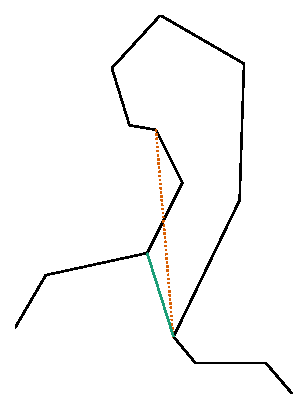
\includegraphics[width=\textwidth]{fig6-selfcrossing-before}
        \caption{Bend's baseline (dotted) is crossing a neighboring bend.}
    \end{subfigure}
    \hfill
    \begin{subfigure}[b]{.49\textwidth}
        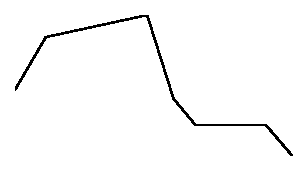
\includegraphics[width=\textwidth]{fig6-selfcrossing-after}
        \caption{Self-crossing removed.}
    \end{subfigure}
    \caption{Originally figure 6: simple case of self-line crossing.}
    \label{fig:fig6-selfcrossing}
\end{figure}

\begin{figure}[h]
    \centering
    \begin{subfigure}[b]{.49\textwidth}
        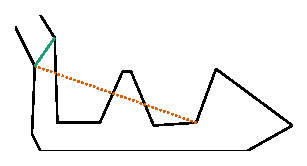
\includegraphics[width=\textwidth]{selfcrossing-1-before}
        \caption{Bend's baseline (dotted) is crossing a non-neighboring bend.}
    \end{subfigure}
    \hfill
    \begin{subfigure}[b]{.49\textwidth}
        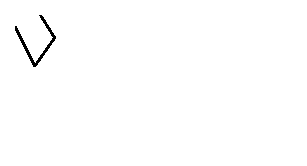
\includegraphics[width=\textwidth]{selfcrossing-1-after}
        \caption{Self-crossing removed.}
    \end{subfigure}
    \caption{Self-crossing with non-neighboring bend.}
    \label{fig:selfcrossing-1-non-neighbor}
\end{figure}

Looking at the {\WM} paper alone, it may seem like self-crossing may happen
only with the neighboring bend. This would mean an efficient $O(n)$
implementation\footnote{where $n$ is the number of bends in a line. See
explanation of \textsc{algorithmic complexity} in section~\ref{sec:vocab}.}.
However, as one can see in figure~\ref{fig:selfcrossing-1-non-neighbor}, it may
not be the case: any other bend in the line may be crossing it.

If one translates the requirements to code in a straightforward way, it would
be quite computationally expensive: naively implemented, complexity of checking
every bend with every bend is $O(n^2)$. In other words, the time it takes to
run the algorithm grows quadratically with the with the number of vertices.

It is possible to optimize this step and skip checking most of the bends. Only
bends whose sum of inner angles is larger than $\pi$ can ever self-cross. If
the value is less than $\pi$, it cannot cross other bends. That way, only a
fraction of bends need to be checked. The worst-case complexity is still
$O(n^2)$, when all bends' inner angles are larger than $\pi$, but, assuming no
more than $20\%$ of the bends' inner angles are larger than $\pi$, the time it
takes to run this piece of the algorithm drops by $80\%$.

\subsection{Attributes of a Single Bend}


\textsc{Compactness Index} is "the ratio of the area of the polygon over the
circle whose circumference length is the same as the length of the
circumference of the polygon" \cite{wang1998line}. Given a bend, its
compactness index is calculated as follows:

\begin{enumerate}

  \item Construct a polygon by joining first and last vertices of the bend.

  \item Calculate area of the polygon.

  \item Calculate perimeter $u$ of the polygon. The same value is the
      circumference of the circle.

  \item Given circle's perimeter $u$, circle's area $A$ is:

    \[
      A = \frac{u^2}{4\pi}
    \]

  \item Compactness index is $\nicefrac{P}{A}$:

    \[
      cmp = \frac{P}{A} = \frac{P}{ \frac{u^2}{4\pi} } = \frac{4\pi P}{u^2}
    \]

\end{enumerate}

Other than that, once this section is implemented, each bend will have a list
of properties, upon which actions later will be performed.

\subsection{Shape of a Bend}

This section introduces \textsc{adjusted size}, which trivially derives from
\textsc{compactness index} $cmp$ and shape's area $A$:

\[
    adjsize = \frac{0.75 A}{cmp}
\]

Adjusted size becomes necessary later to compare bends with each other, and
find out similar ones.

\subsection{Isolated Bend}

Bend itself and its "isolation" can be described by \textsc{average curvature},
which is \textcquote{wang1998line}{geometrically defined as the ratio of
inflection over the length of a curve.}

Two conditions must be true to claim that a bend is isolated:

\begin{enumerate}
    \item \textsc{average curvature} of neighboring bends, should be larger
        than the "candidate" bend's curvature. The article did not offer a
        value, this implementation arbitrarily chose $\isolationThreshold$.

    \item Bends on both sides of the "candidate" should be longer than a
        certain value. This implementation does not (yet) define such a
        constraint and will only follow the average curvature constraint above.
\end{enumerate}

\subsection{The Context of a Bend: Isolated and Similar Bends}

To find out whether two bends are similar, they are compared by 3 components:

\begin{enumerate}
    \item \textsc{adjusted size}
    \item \textsc{compactness index}
    \item Baseline length
\end{enumerate}

Components 1, 2 and 3 represent a point in a 3-dimensional space, and Euclidean
distance $d$ between those is calculated to differentiate between bends $p$ and
$q$:

\[
    d(p,q) = \sqrt{(adjsize_p-adjsize_q)^2 +
                   (cmp_p-cmp_q)^2 +
                   (baseline_p-baseline_q)^2}
\]

The smaller the distance $d$, the more similar the bends are.

\subsection{Elimination Operator}

\subsection{Combination Operator}

\subsection{Exaggeration Operator}

\section{Program Implementation}

\section{Results of Experiments}

\section{Conclusions}
\label{sec:conclusions}

\section{Related Work and future suggestions}
\label{sec:related_work}

\printbibliography

\begin{appendices}

\section{Code listings}

\subsection{Re-generating this paper}
\label{sec:code-regenerate}

Like explained in section~\ref{sec:reproducing-the-paper}, illustrations in
    this paper are generated from a small list of sample geometries. To observe
    the source geometries or regenerate this paper, run this script (assuming
    name of this document is {\tt mj-msc-full.pdf}):

\inputcode{bash}{extract-and-generate}

%\subsection{Algorithm code listings}
%\inputcode{postgresql}{wm.sql}

\end{appendices}
\end{document}
